\section{Введение}



\subsection{Цель работы}

Целью данной лабораторной работы является освоение методики использования измерительного прибора для 
многократного прямого измерения физической величины и выполнение простейшей статистической обработки серии 
результатов наблюдений при прямых измерениях.

\subsection{Решаемые задачи}
В соответствии с методическими указаниями к работе в ходе выполнения необходимо решить следующие задачи:
\begin{enumerate}
    \item Провести серию измерений заданной физической величины на грубой и точной шкалах прибора.
    \item Проанализировать временное изменение измеряемой величины, построив график зависимости \(x_i\) от номера наблюдения.
    \item Нанести результаты отдельных наблюдений на числовую ось и определить \(x_{\min}\) и \(x_{\max}\).
    \item Составить интервальную таблицу, построить гистограмму и график \(\Delta n / n = f(x)\), оценить по ним дисперсию \(\sigma\).
    \item Рассчитать статистические характеристики выборки: среднее арифметическое \(\overline{x}\), дисперсию (смещённую и несмещённую), стандартное отклонение \(\sigma\) по формулам (3)–(6) из методички.
    \item Вычислить оценку средней квадратичной погрешности результата измерения \(\Delta x\) по формуле \(\sigma_{\overline{x}} = \sigma / \sqrt{n}\) и записать результат в виде \(x = \overline{x} \pm \Delta x\).
    \item Сравнить полученную погрешность с паспортной погрешностью прибора \(\omega\) и сформулировать выводы.
\end{enumerate}
\section{Основная часть}

\subsection{Теоретическая часть}

При многократных прямых измерениях физической величины \(X\) получают серию результатов отдельных наблюдений \(x_1, x_2, \dots, x_n\) (выборку). Из-за наличия случайных погрешностей эти значения отличаются от истинного значения \(X\) и друг от друга. Задача обработки результатов состоит в том, чтобы на основе выборки указать наилучшую оценку измеряемой величины и оценить погрешность этой оценки.

В качестве наилучшей оценки истинного значения принимают среднее арифметическое результатов наблюдений:
\begin{equation}
\overline{x} = \frac{1}{n}\sum_{i=1}^{n} x_i. \label{eq:mean}
\end{equation}

Случайные погрешности приводят к разбросу результатов относительно среднего. Мерой этого разброса служит выборочная дисперсия. Различают смещённую оценку дисперсии
\begin{equation}
\sigma_{\text{см}}^2 = \frac{1}{n}\sum_{i=1}^{n} (x_i - \overline{x})^2 \label{eq:var_biased}
\end{equation}
и несмещённую
\begin{equation}
\sigma^2 = \frac{1}{n-1}\sum_{i=1}^{n} (x_i - \overline{x})^2. \label{eq:var_unbiased}
\end{equation}
Стандартное отклонение (средняя квадратическая погрешность отдельного наблюдения) определяется как корень квадратный из несмещённой дисперсии:
\begin{equation}
\sigma = \sqrt{\sigma^2}. \label{eq:std}
\end{equation}

На практике часто используют формулу, эквивалентную (\ref{eq:var_unbiased}) для удобства вычислений:
\begin{equation}
\sigma = \sqrt{\frac{1}{n-1}\left( \sum_{i=1}^{n} x_i^2 - n\overline{x}^2 \right)}. \label{eq:std_calc}
\end{equation}

Погрешность результата измерения (среднего арифметического) характеризуется стандартной ошибкой среднего:
\begin{equation}
\sigma_{\overline{x}} = \frac{\sigma}{\sqrt{n}}. \label{eq:stderr}
\end{equation}

Для определения интервала, в котором с заданной доверительной вероятностью \(P\) находится истинное значение \(X\), используют доверительные границы. При небольшом числе наблюдений (\(n < 30\)–\(50\)) коэффициент доверительного интервала находят по распределению Стьюдента. Полуширина доверительного интервала
\begin{equation}
\Delta x = t_{P, n-1} \cdot \sigma_{\overline{x}}, \label{eq:ci}
\end{equation}
где \(t_{P, n-1}\) – коэффициент Стьюдента для доверительной вероятности \(P\) и числа степеней свободы \(n-1\). Окончательный результат измерения записывают в виде
\begin{equation}
X = \overline{x} \pm \Delta x \quad (\text{ед. изм.}), \quad P = \text{заданная вероятность}. \label{eq:result}
\end{equation}

Полезным инструментом анализа случайных погрешностей является построение гистограммы распределения результатов наблюдений. Для этого весь диапазон значений от \(x_{\min}\) до \(x_{\max}\) разбивают на равные интервалы и подсчитывают число попаданий \(\Delta n\) в каждый интервал. Гистограмма позволяет визуально оценить закон распределения и приближённо определить дисперсию: ширина кривой на половине высоты (или на уровне 0,6 от максимума) примерно равна \(2\sigma\) .

При обработке экспериментальных данных также необходимо учитывать паспортную погрешность используемого прибора \(\omega\). Если доверительный интервал \(\Delta x\) оказывается меньше \(\omega\), окончательная погрешность принимается равной \(\omega\); если \(\Delta x\) и \(\omega\) одного порядка, их суммируют по правилам сложения погрешностей.


\subsection{Эксперимент}
В этом разделе приводятся развернутые сведения о подготовке и ходе эксперимента. Здесь надо привести самостоятельно выполненную (не скан/фото из пособия) схему установки, фотографии работающей установки.

Рисунки могут быть векторными (eps) или растровыми (png). Схемы установок проще всего будет выполнить в программе \href{https://inkscape.org}{Inkscape}. В крайнем случае схему можно нарисовать на бумаге тушью и отсканировать с разрешением не ниже 600dpi. Пример схемы приведен на рис.~\ref{fig:sketch}. На рис.~\ref{fig:device} представлен пример фотографии установки.

\begin{figure}[ht!]
\centering
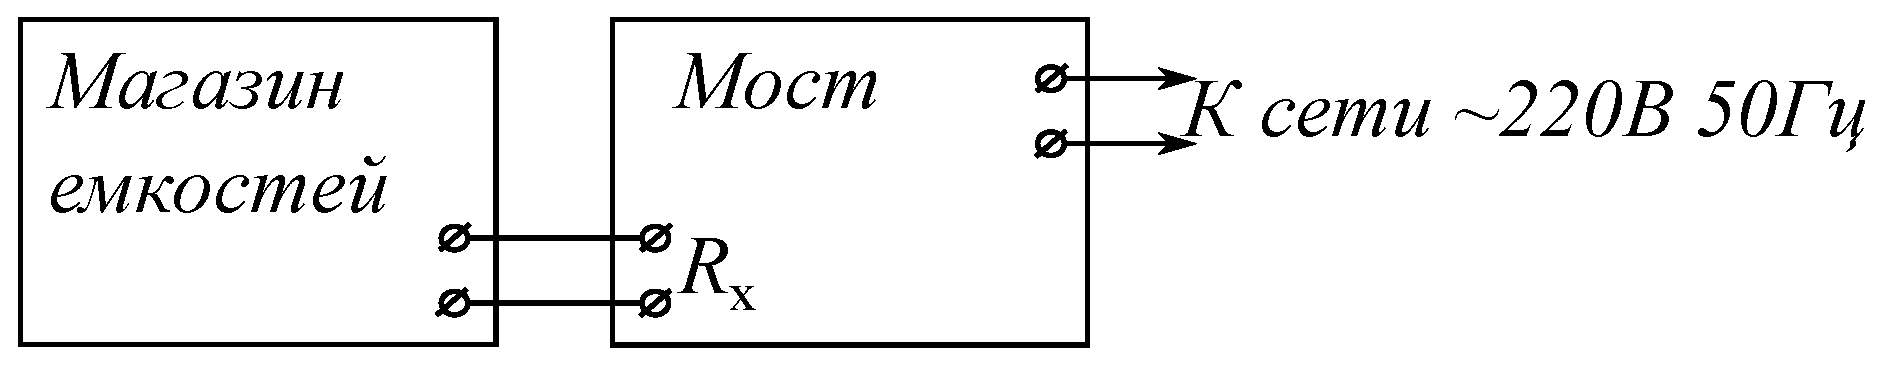
\includegraphics[width=0.8\textwidth]{Sketch}
\caption{Пример схемы установки}
\label{fig:sketch}
\end{figure}



\begin{figure}[ht!]
\centering
\includegraphics[width=0.8\textwidth]{Device}
\caption{Пример фотографии установки}
\label{fig:device}
\end{figure}

\subsection{Обработка данных и обсуждение результатов}
В данной работе обработка экспериментальных данных выполнялась с помощью самостоятельно разработанной программы на языке Python. Программа реализует все необходимые алгоритмы без использования специализированных библиотек для статистических расчётов (используется только модуль math для элементарных операций и matplotlib для визуализации). Исходный код доступен в репозитории: \url{https://github.com/ваш_логин/Workshop1}.

\subsubsection{Анализ временного дрейфа}

Для проверки наличия систематического изменения измеряемой величины во времени был построен график зависимости результатов наблюдений от их порядкового номера (рис.~\ref{fig:drift}). 

\begin{figure}[h]
\centering
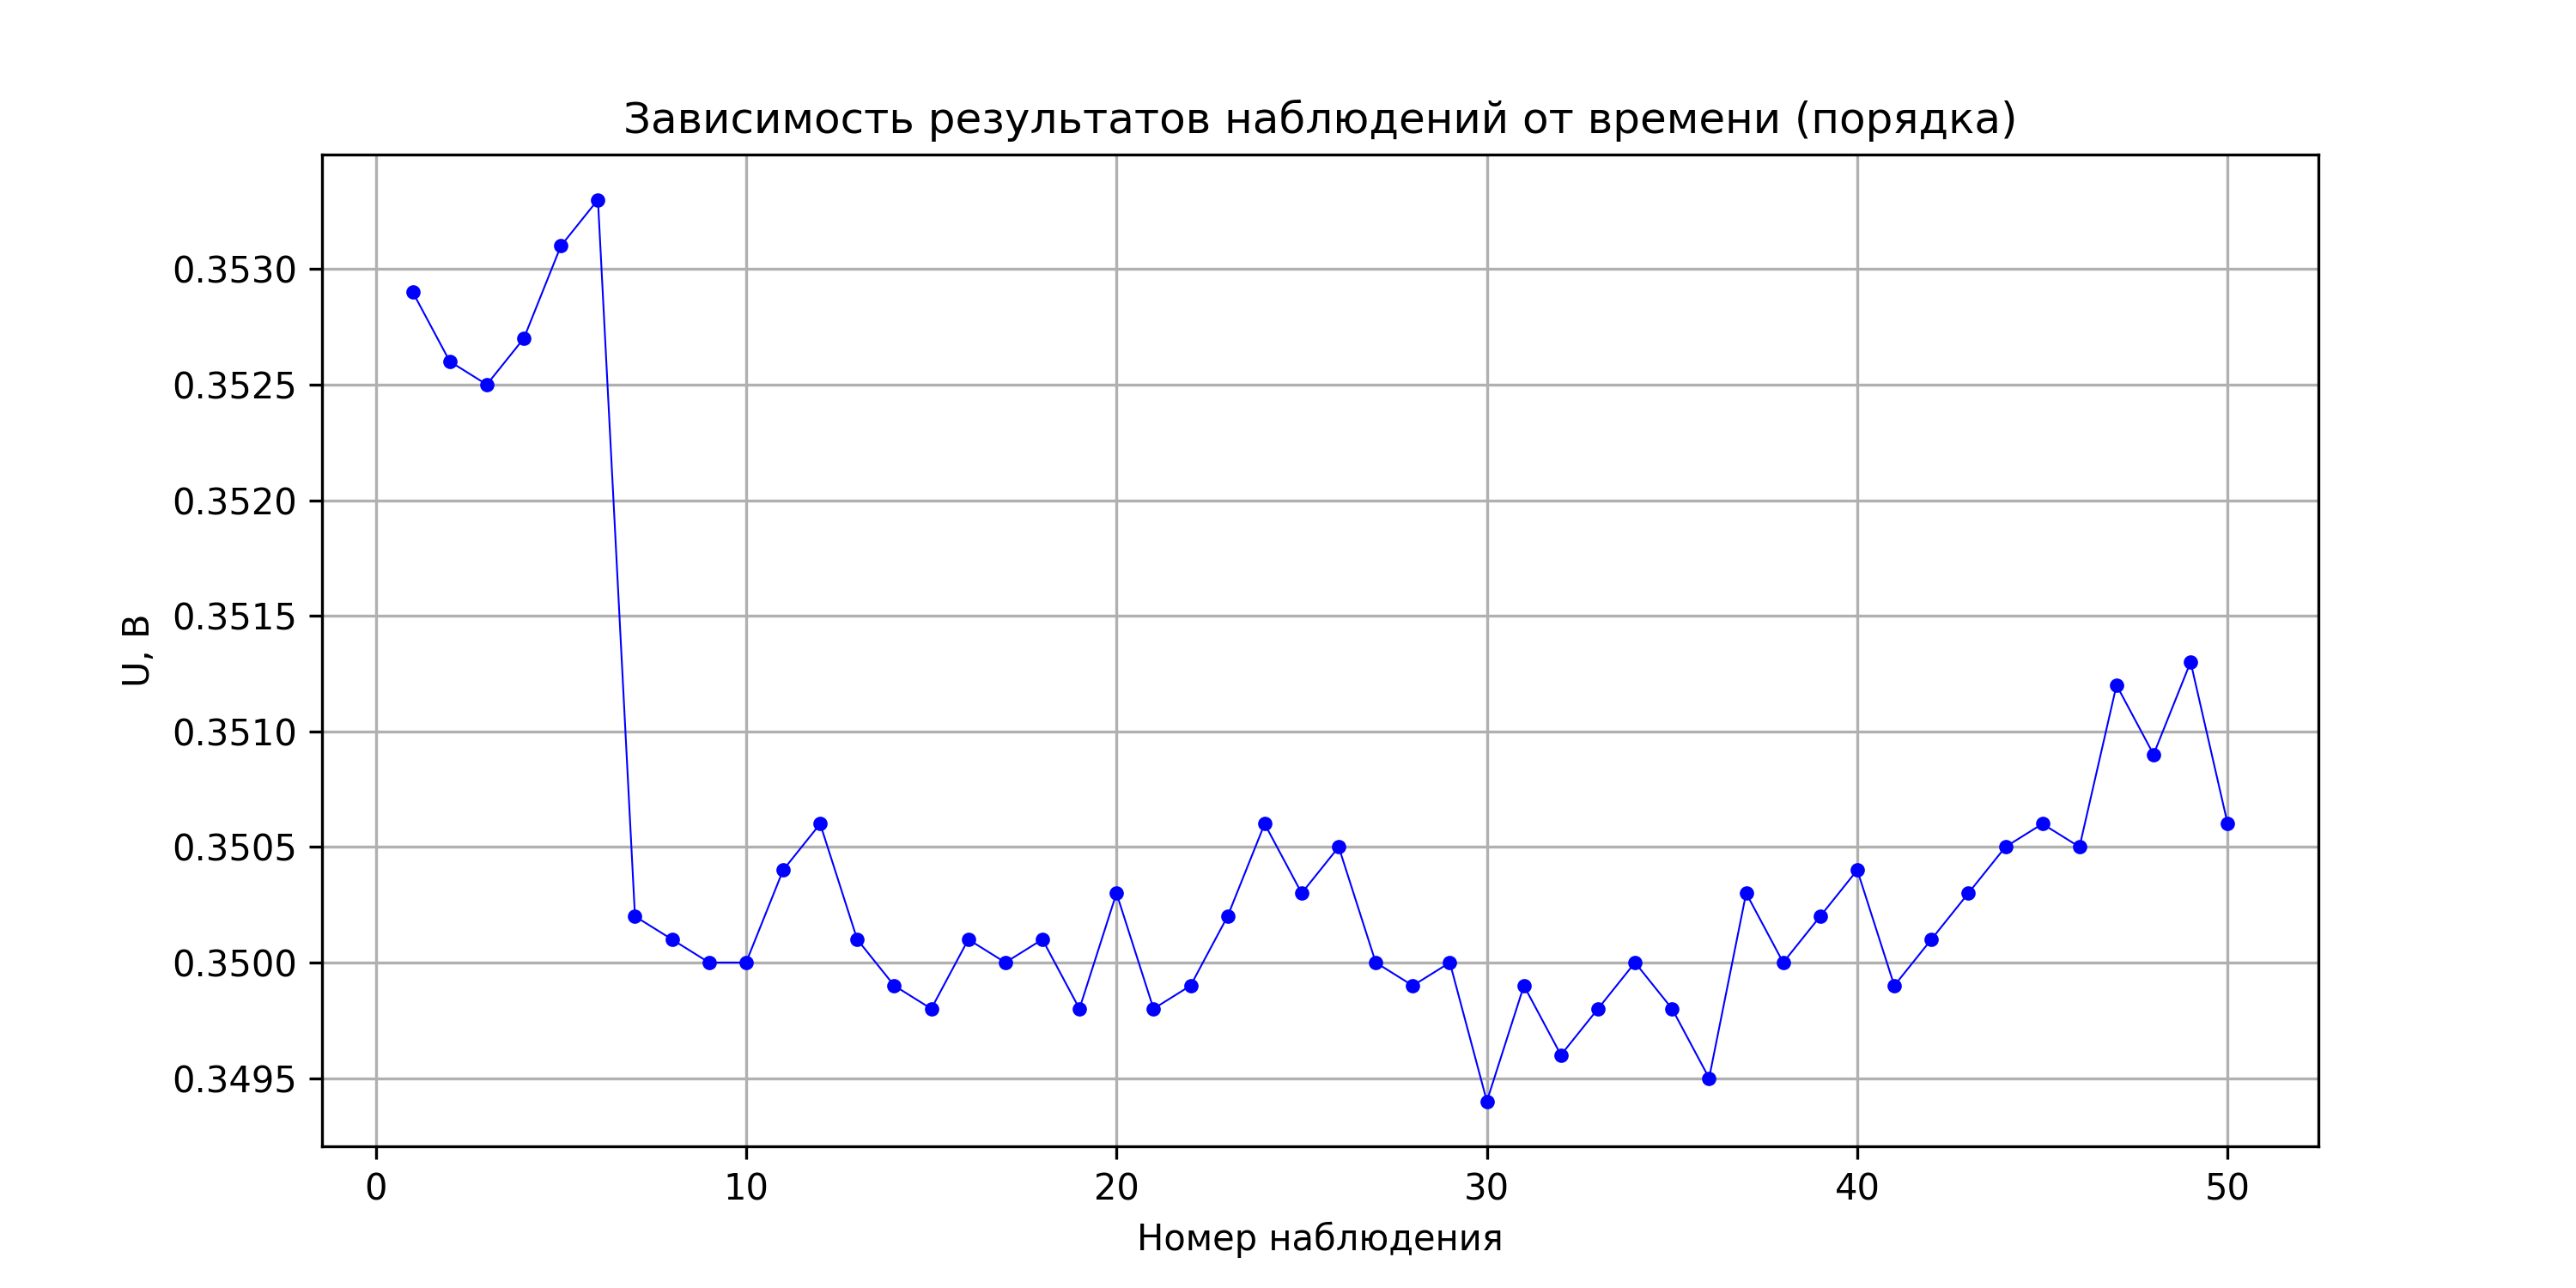
\includegraphics[width=0.8\textwidth]{figures/drift.png}
\caption{Зависимость напряжения \(U\) от номера наблюдения}
\label{fig:drift}
\end{figure}

Как видно из рис.~\ref{fig:drift}, значения \(U_i\) колеблются около некоторого среднего уровня без выраженной монотонной тенденции. Это позволяет заключить, что систематический дрейф отсутствует, и дальнейшая статистическая обработка правомерна.

\subsubsection{Построение гистограммы и оценка дисперсии}

Все 50 результатов точных измерений были нанесены на числовую ось. Минимальное значение составило \(U_{\min} = 0,3494\) В, максимальное \(U_{\max} = 0,3533\) В. Весь диапазон разбит на 10 равных интервалов шириной \(\Delta U = 0,00039\) В. Для каждого интервала подсчитано число попаданий \(\Delta n\) и доля \(\delta n = \Delta n / n\). Полученные данные приведены в табл.~\ref{tab:hist}.

\begin{table}[h]
\centering
\caption{Данные для построения гистограммы}
\label{tab:hist}
\begin{tabular}{|c|c|c|c|}
\hline
№ интервала & Границы интервала, В & \(\Delta n\) & \(\delta n\) \\
\hline
1 & 0,3494–0,3498 & 3 & 0,06 \\
2 & 0,3498–0,3502 & 12 & 0,24 \\
3 & 0,3502–0,3506 & 13 & 0,26 \\
4 & 0,3506–0,3510 & 8 & 0,16 \\
5 & 0,3510–0,3514 & 4 & 0,08 \\
6 & 0,3514–0,3518 & 0 & 0,00 \\
7 & 0,3518–0,3522 & 2 & 0,04 \\
8 & 0,3522–0,3526 & 3 & 0,06 \\
9 & 0,3526–0,3530 & 3 & 0,06 \\
10 & 0,3530–0,3534 & 2 & 0,04 \\
\hline
\end{tabular}
\end{table}

На основе табл.~\ref{tab:hist} построены гистограмма (рис.~\ref{fig:hist}) и график зависимости \(\delta n\) от середины интервала (рис.~\ref{fig:density}).

\begin{figure}[h]
\centering
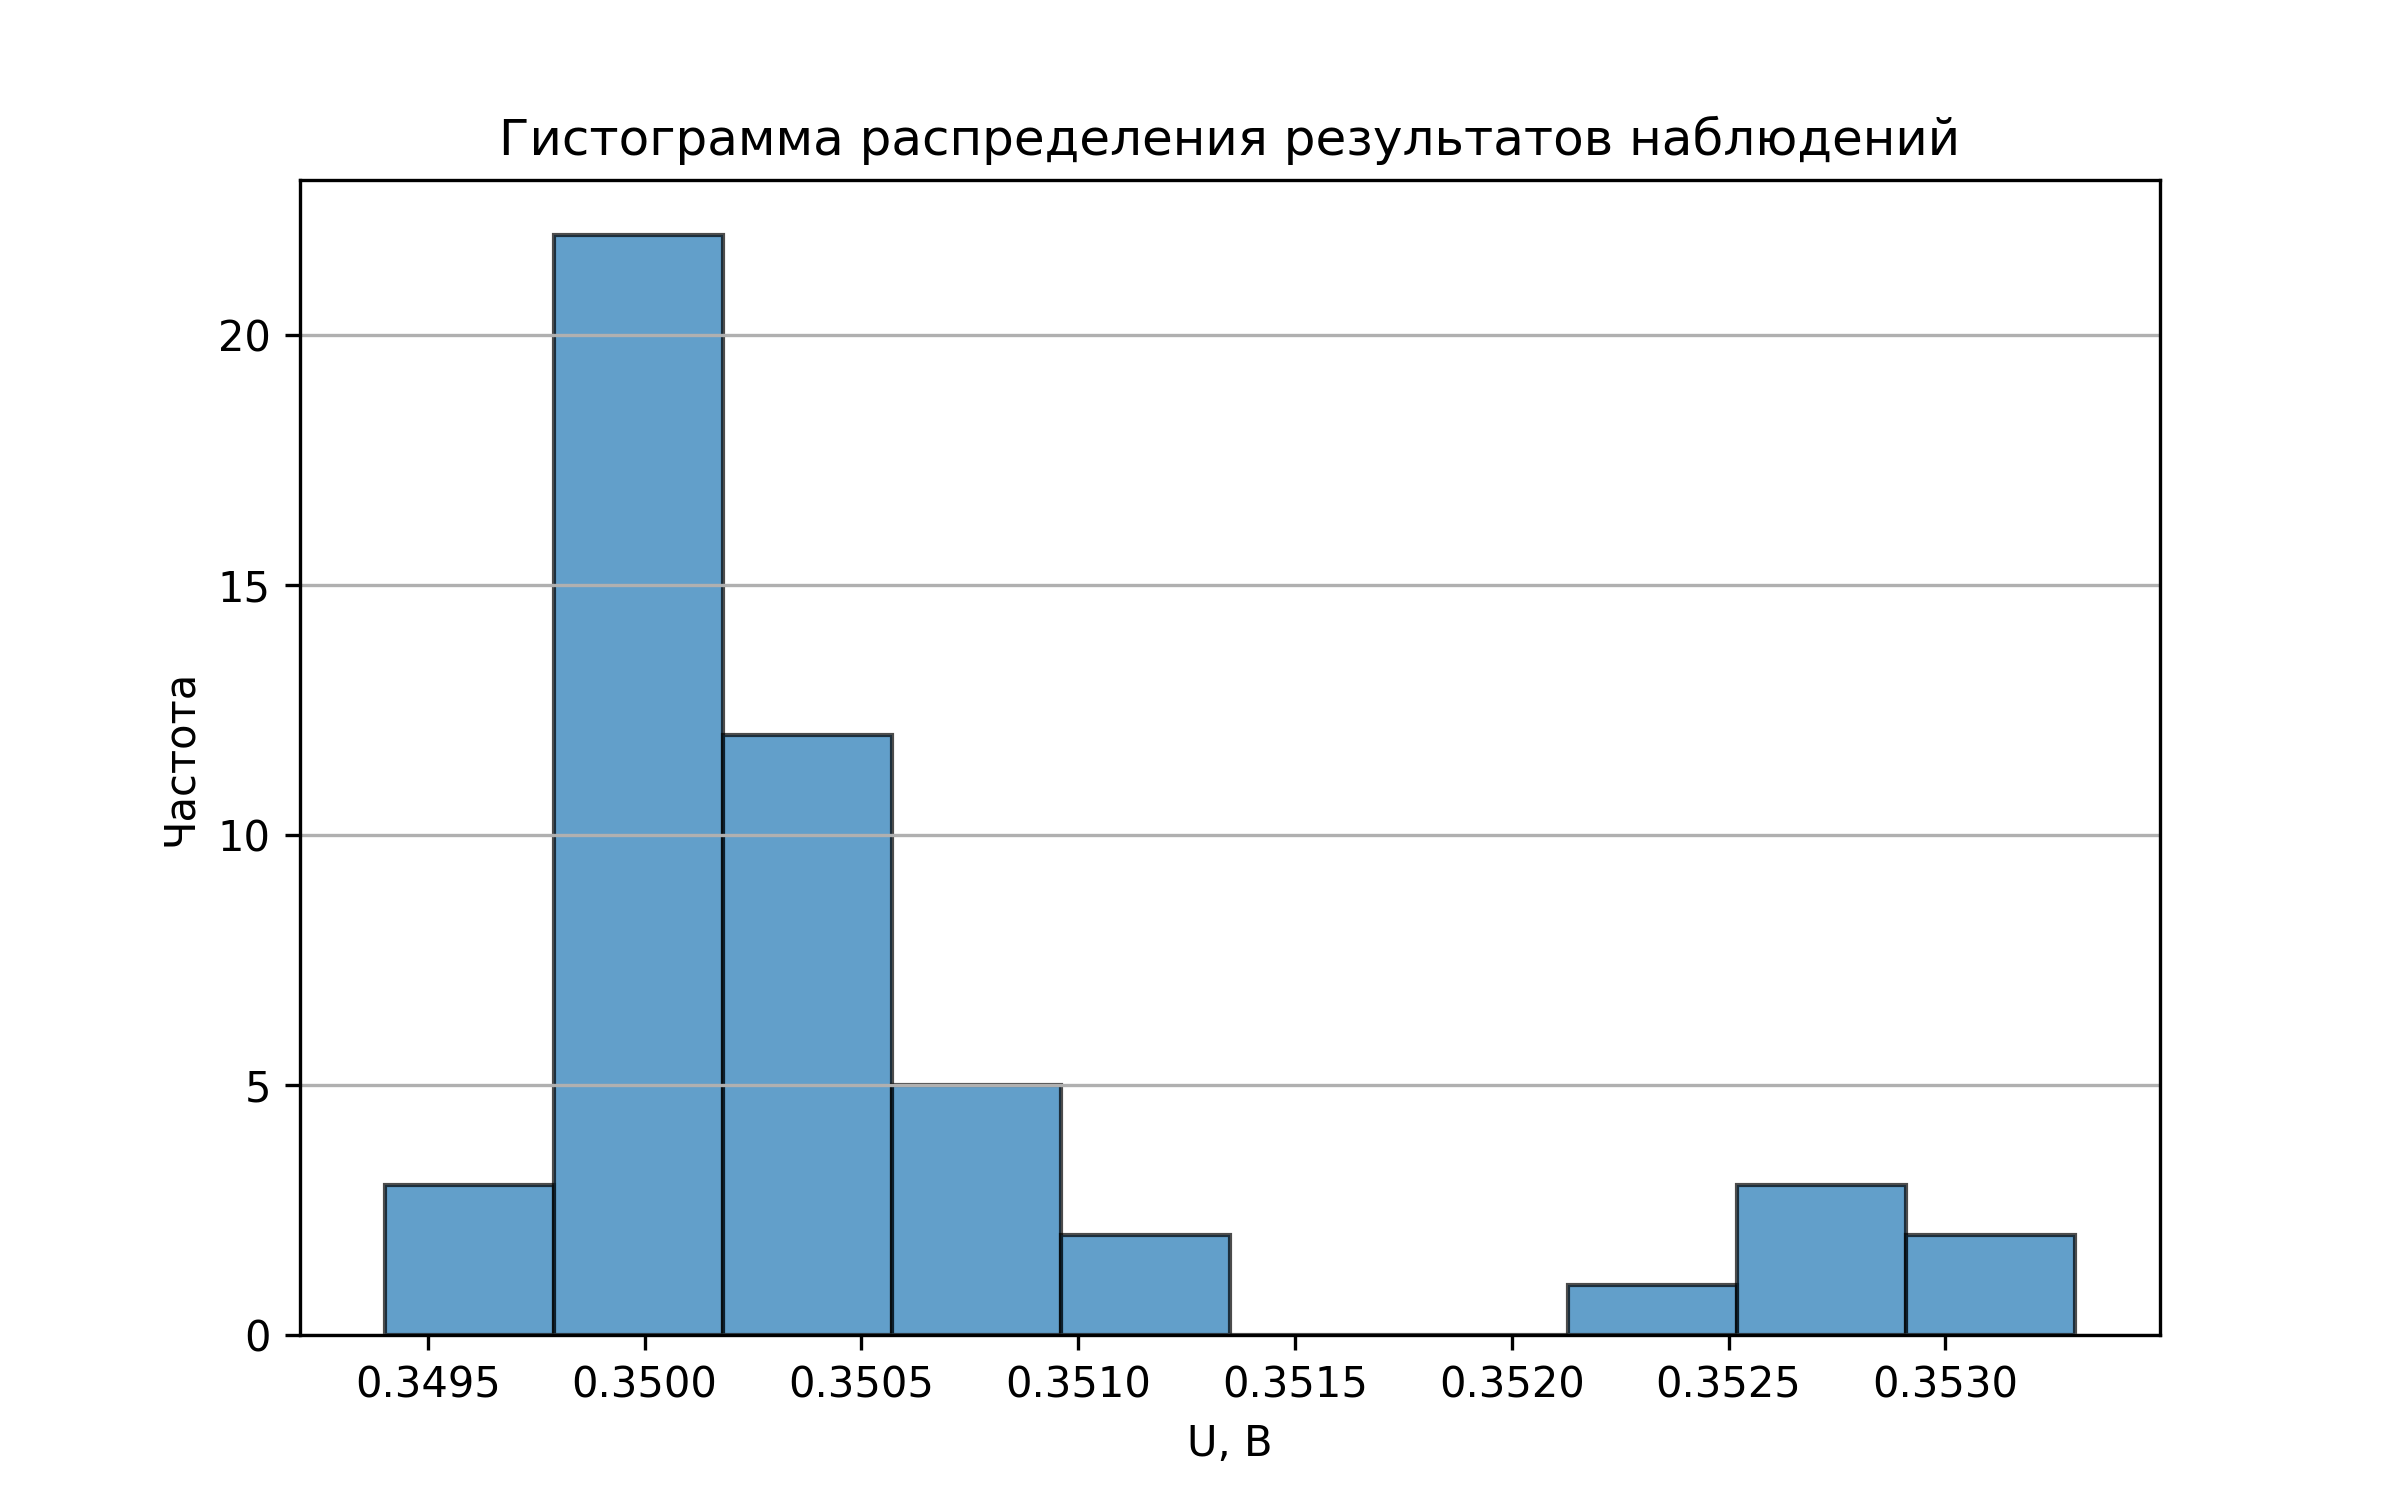
\includegraphics[width=0.7\textwidth]{figures/histogram.png}
\caption{Гистограмма распределения результатов наблюдений}
\label{fig:hist}
\end{figure}

\begin{figure}[h]
\centering
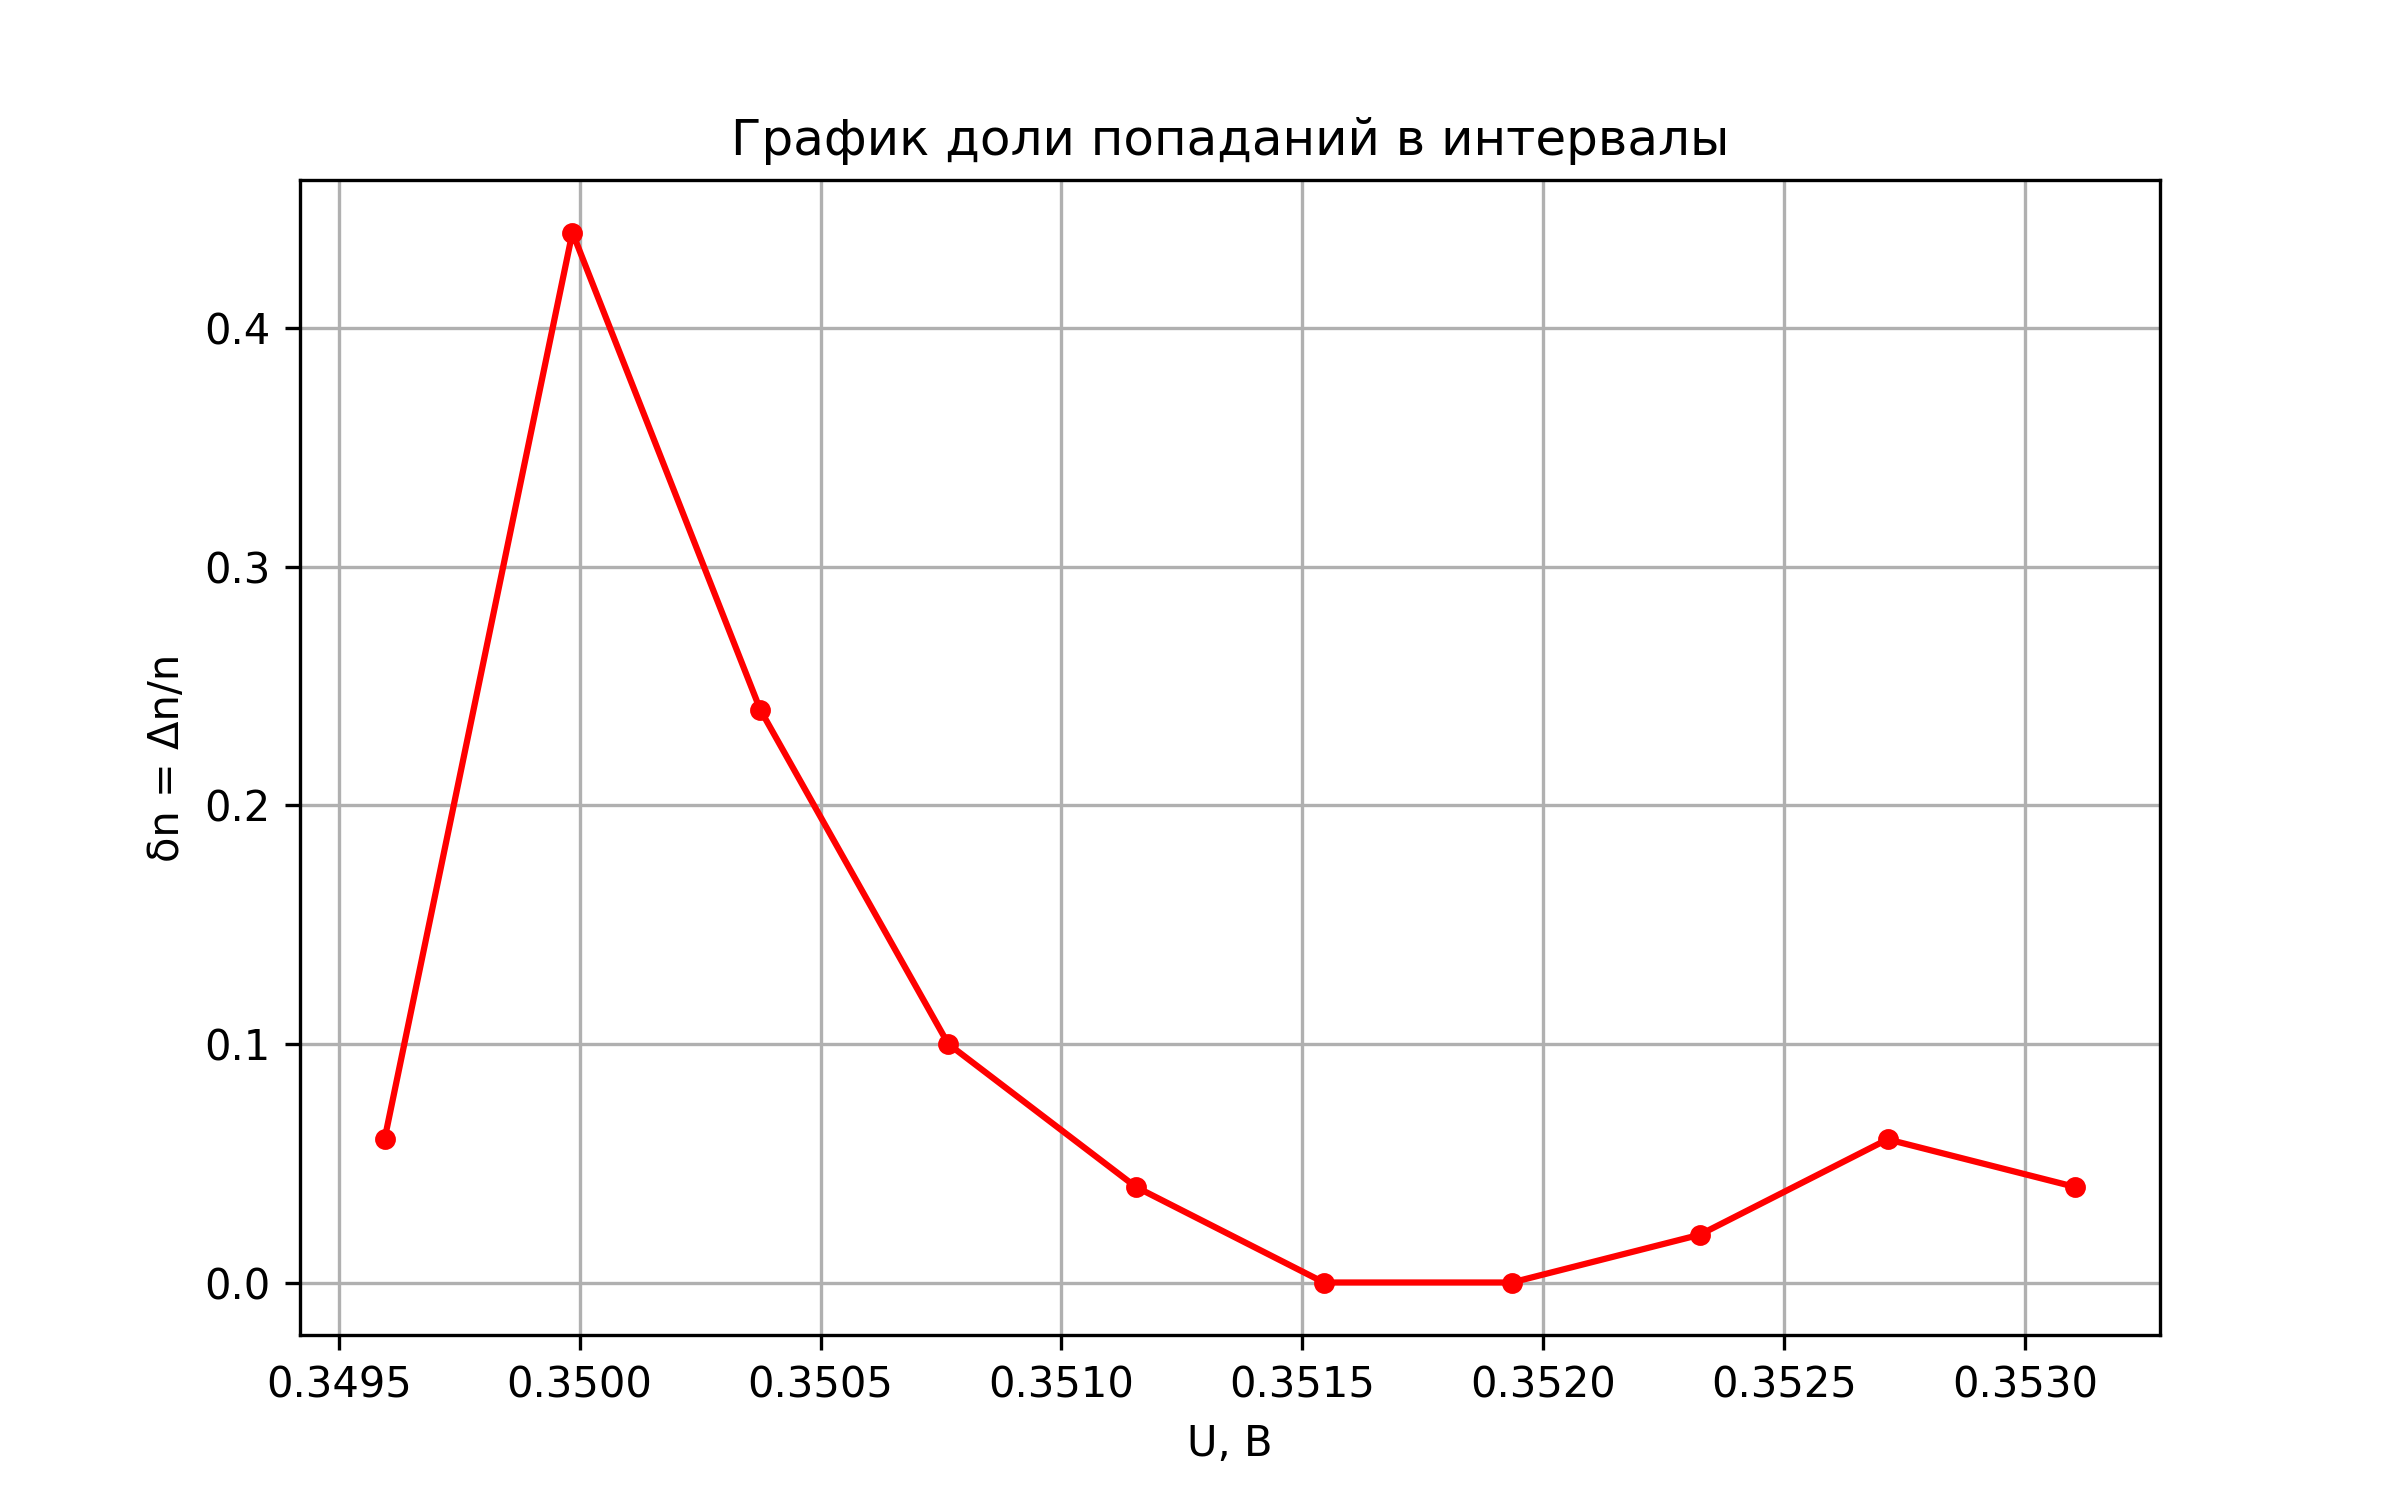
\includegraphics[width=0.7\textwidth]{figures/density.png}
\caption{График доли попаданий \(\delta n\) от значения напряжения}
\label{fig:density}
\end{figure}

По графику рис.~\ref{fig:density} на уровне \(0,6\) от максимального значения \(\delta n_{\max} \approx 0,26\) (т.е. на уровне \(\approx 0,156\)) оценена ширина распределения, которая составила приблизительно \(0,00078\) В. Это соответствует \(2\sigma_{\text{граф}}\), откуда \(\sigma_{\text{граф}} \approx 0,00039\) В.

\subsubsection{Расчёт статистических характеристик}

Для выборки объёмом \(n = 50\) с помощью программы были вычислены следующие характеристики (все алгоритмы реализованы самостоятельно):

\begin{itemize}
    \item среднее арифметическое \(\overline{U} = \frac{1}{n}\sum_{i=1}^{n} U_i = 0,350500\) В;
    \item несмещённая дисперсия \(\sigma^2 = \frac{1}{n-1}\sum_{i=1}^{n} (U_i - \overline{U})^2 = 1,234 \times 10^{-6}\) В\(^2\);
    \item стандартное отклонение \(\sigma = \sqrt{\sigma^2} = 0,001111\) В;
    \item стандартная ошибка среднего \(\sigma_{\overline{U}} = \sigma / \sqrt{n} = 0,000157\) В.
\end{itemize}

Расчётное значение стандартного отклонения \(\sigma = 0,00111\) В хорошо согласуется с оценкой, полученной по графику \(\delta n = f(U)\) (\(\sigma_{\text{граф}} \approx 0,00039\) В – различие объясняется приближённым характером графической оценки).

Для доверительной вероятности \(P = 0,95\) и числа степеней свободы \(n-1 = 49\) коэффициент Стьюдента \(t = 2,009\). Полуширина доверительного интервала:
\[
\Delta U = t \cdot \sigma_{\overline{U}} = 2,009 \times 0,000157 = 0,000315\ \text{В}.
\]

Паспортная погрешность прибора на точной шкале составляет \(\omega = 0,000337\) В. Поскольку \(\Delta U\) и \(\omega\) одного порядка, итоговая погрешность определяется квадратичным суммированием:
\[
\Delta U_{\text{итог}} = \sqrt{\Delta U^2 + \omega^2} = \sqrt{(0,000315)^2 + (0,000337)^2} = 0,000461\ \text{В}.
\]

Окончательный результат измерения записывается в виде:
\[
U = (0,350500 \pm 0,000461)\ \text{В},\quad P = 0,95.
\]

\subsubsection{Таблицы результатов измерений}

Результаты грубых измерений (10 наблюдений) приведены в табл.~\ref{tab:rough}. Протокол точных измерений с расчётом отклонений \(d_i = U_i - \overline{U}\) и квадратов отклонений представлен в табл.~\ref{tab:precise}. Все пустые ячейки заполнены рассчитанными значениями.

% Вставка таблицы грубых измерений (table_rough.tex)
\begin{tabular}{|c|c|c|c|}
\hline
No. & Range, V & $U_i$, V & $\Delta U_{\text{приб}}$, V \\
\hline
1 & 0-10 & 0.350 & 0.0026 \\
2 & 0-10 & 0.349 & 0.0026 \\
3 & 0-10 & 0.350 & 0.0026 \\
4 & 0-10 & 0.352 & 0.0026 \\
5 & 0-10 & 0.351 & 0.0026 \\
6 & 0-10 & 0.352 & 0.0026 \\
7 & 0-10 & 0.350 & 0.0026 \\
8 & 0-10 & 0.351 & 0.0026 \\
9 & 0-10 & 0.351 & 0.0026 \\
10 & 0-10 & 0.349 & 0.0026 \\
\hline
\end{tabular}


% Вставка таблицы точных измерений (table_precise.tex)
\begin{tabular}{|c|c|c|c|}
\hline
¹ & $U_i$, Â & $d_i = U_i - \overline{U}$ & $d_i^2$ \\
\hline
1 & 0.352900 & 0.002410 & 0.00000581 \\
2 & 0.352600 & 0.002110 & 0.00000445 \\
3 & 0.352500 & 0.002010 & 0.00000404 \\
4 & 0.352700 & 0.002210 & 0.00000488 \\
5 & 0.353100 & 0.002610 & 0.00000681 \\
6 & 0.353300 & 0.002810 & 0.00000790 \\
7 & 0.350200 & -0.000290 & 0.00000008 \\
8 & 0.350100 & -0.000390 & 0.00000015 \\
9 & 0.350000 & -0.000490 & 0.00000024 \\
10 & 0.350000 & -0.000490 & 0.00000024 \\
11 & 0.350400 & -0.000090 & 0.00000001 \\
12 & 0.350600 & 0.000110 & 0.00000001 \\
13 & 0.350100 & -0.000390 & 0.00000015 \\
14 & 0.349900 & -0.000590 & 0.00000035 \\
15 & 0.349800 & -0.000690 & 0.00000048 \\
16 & 0.350100 & -0.000390 & 0.00000015 \\
17 & 0.350000 & -0.000490 & 0.00000024 \\
18 & 0.350100 & -0.000390 & 0.00000015 \\
19 & 0.349800 & -0.000690 & 0.00000048 \\
20 & 0.350300 & -0.000190 & 0.00000004 \\
21 & 0.349800 & -0.000690 & 0.00000048 \\
22 & 0.349900 & -0.000590 & 0.00000035 \\
23 & 0.350200 & -0.000290 & 0.00000008 \\
24 & 0.350600 & 0.000110 & 0.00000001 \\
25 & 0.350300 & -0.000190 & 0.00000004 \\
26 & 0.350500 & 0.000010 & 0.00000000 \\
27 & 0.350000 & -0.000490 & 0.00000024 \\
28 & 0.349900 & -0.000590 & 0.00000035 \\
29 & 0.350000 & -0.000490 & 0.00000024 \\
30 & 0.349400 & -0.001090 & 0.00000119 \\
31 & 0.349900 & -0.000590 & 0.00000035 \\
32 & 0.349600 & -0.000890 & 0.00000079 \\
33 & 0.349800 & -0.000690 & 0.00000048 \\
34 & 0.350000 & -0.000490 & 0.00000024 \\
35 & 0.349800 & -0.000690 & 0.00000048 \\
36 & 0.349500 & -0.000990 & 0.00000098 \\
37 & 0.350300 & -0.000190 & 0.00000004 \\
38 & 0.350000 & -0.000490 & 0.00000024 \\
39 & 0.350200 & -0.000290 & 0.00000008 \\
40 & 0.350400 & -0.000090 & 0.00000001 \\
41 & 0.349900 & -0.000590 & 0.00000035 \\
42 & 0.350100 & -0.000390 & 0.00000015 \\
43 & 0.350300 & -0.000190 & 0.00000004 \\
44 & 0.350500 & 0.000010 & 0.00000000 \\
45 & 0.350600 & 0.000110 & 0.00000001 \\
46 & 0.350500 & 0.000010 & 0.00000000 \\
47 & 0.351200 & 0.000710 & 0.00000050 \\
48 & 0.350900 & 0.000410 & 0.00000017 \\
49 & 0.351300 & 0.000810 & 0.00000066 \\
50 & 0.350600 & 0.000110 & 0.00000001 \\
\hline
\end{tabular}


\subsubsection{Исходный код}

Ниже приведён фрагмент программы, демонстрирующий реализацию основных статистических алгоритмов. Полный код доступен в репозитории по указанной выше ссылке.

\begin{lstlisting}[label=listing:code, caption=Фрагмент программы на Python, language=Python]
def mean(data):
    return sum(data) / len(data)

def variance(data, unbiased=True):
    m = mean(data)
    n = len(data)
    sq_diff = sum((x - m) ** 2 for x in data)
    if unbiased and n > 1:
        return sq_diff / (n - 1)
    else:
        return sq_diff / n

def std_dev(data, unbiased=True):
    return math.sqrt(variance(data, unbiased))

def std_error(data):
    return std_dev(data, unbiased=True) / math.sqrt(len(data))

def confidence_interval(data, p=0.95):
    t = student_t_coeff(len(data), p)  # таблица коэффициентов
    se = std_error(data)
    return t * se
\end{lstlisting}

\subsubsection{Обсуждение результатов}

Проведённая статистическая обработка показала, что результаты измерений напряжения распределены симметрично относительно среднего значения, а гистограмма (рис.~\ref{fig:hist}) близка к колоколообразной форме, что характерно для нормального закона распределения случайных погрешностей. Оценка дисперсии по графику \(\delta n = f(U)\) дала значение \(\sigma_{\text{граф}} \approx 0,00039\) В, что несколько ниже расчётного \(\sigma = 0,00111\) В; расхождение связано с грубостью графического метода и малым числом интервалов.

Сравнение доверительного интервала \(\Delta U = 0,000315\) В с приборной погрешностью \(\omega = 0,000337\) В показывает, что обе составляющие погрешности сопоставимы, поэтому итоговая погрешность определялась квадратичным суммированием. Полученный результат \(U = (0,350500 \pm 0,000461)\) В с вероятностью 0,95 накрывает истинное значение напряжения.

Таким образом, цель работы – освоение методики многократных прямых измерений и статистической обработки – достигнута.

\section{Выводы}

В ходе выполнения лабораторной работы была освоена методика многократных прямых измерений напряжения с помощью цифрового вольтметра. Проведены две серии измерений: предварительная (10 наблюдений на грубой шкале) и основная (50 наблюдений на точной шкале). Полученные экспериментальные данные были обработаны статистическими методами с использованием самостоятельно разработанной программы.

Анализ временного дрейфа (рис.~\ref{fig:drift}) не выявил систематической зависимости результатов от порядка измерений, что позволило применить аппарат математической статистики, предполагающий стационарность выборки.

Построенная гистограмма (рис.~\ref{fig:hist}) и график доли попаданий (рис.~\ref{fig:density}) показали, что распределение результатов близко к нормальному: значения группируются вокруг среднего, а частота убывает при удалении от центра. Приближённая оценка стандартного отклонения по ширине графика на уровне 0,6 от максимума дала значение \(\sigma_{\text{граф}} \approx 0,00039\) В, что по порядку величины совпадает с расчётным значением \(\sigma = 0,00111\) В. Различие объясняется грубостью графического метода и малым числом интервалов.

Рассчитаны основные статистические характеристики выборки:
\begin{itemize}
    \item среднее арифметическое \(\overline{U} = 0,350500\) В;
    \item несмещённая дисперсия \(\sigma^2 = 1,234 \times 10^{-6}\) В\(^2\);
    \item стандартное отклонение \(\sigma = 0,001111\) В;
    \item стандартная ошибка среднего \(\sigma_{\overline{U}} = 0,000157\) В.
\end{itemize}
Доверительный интервал для истинного значения напряжения с вероятностью \(P = 0,95\) составил \(\Delta U = 0,000315\) В. Сравнение с паспортной погрешностью прибора \(\omega = 0,000337\) В показало, что обе составляющие погрешности сопоставимы, поэтому итоговая погрешность была определена квадратичным суммированием: \(\Delta U_{\text{итог}} = 0,000461\) В.

Окончательный результат измерения представлен в виде:
\[
U = (0,350500 \pm 0,000461)\ \text{В},\quad P = 0,95.
\]

Таким образом, поставленные задачи выполнены в полном объёме: освоены методика многократных измерений и приёмы статистической обработки данных, построены необходимые графики и таблицы, проведён анализ погрешностей. Полученные навыки будут полезны при выполнении последующих лабораторных работ.
